% Use only LaTeX2e, calling the article.cls class and 12-point type.

\documentclass[11pt]{article}

\usepackage[round,semicolon]{natbib}
\usepackage{etoolbox}
\AtBeginEnvironment{quote}{\singlespacing\tiny}
% Use times if you have the font installed; otherwise, comment out the
% following line.

% added by SKH
%\usepackage{lineno}
%\linenumbers

\usepackage{times}
\usepackage{amssymb}
\usepackage{amsmath}

\usepackage[export]{adjustbox}

\usepackage{graphicx}
\graphicspath{ {images/} }

% for adjustwidth
\usepackage{changepage}

% The following parameters seem to provide a reasonable page setup.

\topmargin 0.0cm
\oddsidemargin 0.2cm
\textwidth 16cm 
\textheight 21cm
\footskip 1.0cm

\usepackage{newfloat}
\usepackage{amsmath}
\usepackage[labelfont=bf]{caption}
\usepackage{nameref}
\usepackage{rotating}
\usepackage{color}
\usepackage{float}
\renewcommand{\figurename}{{}}
\renewcommand{\thefigure}{{Figure \arabic{figure}}}

\renewcommand{\tablename}{{}}
\renewcommand{\thetable}{{Table \arabic{table}}}

\newfloat{suppfile}{thp}{losuppfile}
\renewcommand{\thesuppfile}{Supplementary file \arabic{suppfile}}
\floatname{suppfile}{}

\newfloat{suppfig}{thp}{losuppfig}
\renewcommand{\thesuppfig}{Supplementary figure \arabic{suppfig}}
\floatname{suppfig}{}

%
\newfloat{supptable}{thp}{losupptable}
\renewcommand{\thesupptable}{Supplementary table \arabic{supptable}}
\floatname{supptable}{}
%

\renewcommand{\theequation}{Equation \arabic{equation}}

\newcommand{\mutDNA}{\textbf{mutDNA}}
\newcommand{\mutvirus}{\textbf{mutvirus}}
\newcommand{\DNA}{\textbf{DNA}}
\newcommand{\virus}{\textbf{virus}}

\newcommand\skhcomment[1]{{\color{cyan}#1}}
\newcommand\jdbcomment[1]{{\color{red}#1}}


\usepackage{hyperref}
\hypersetup{colorlinks,citecolor=blue,linkcolor=blue,urlcolor=blue}
\hypersetup{colorlinks,citecolor=blue,linkcolor=blue,urlcolor=blue}

\usepackage{seqsplit}

\usepackage{array}
\newcolumntype{P}[1]{>{\raggedright\arraybackslash}p{#1}}

\title{Experimentally Informed Site-Specific Substitution Models Substantially Deepen Viral Divergence Estimates} 

\author
{Sarah K. Hilton$^{1,2}$  and Jesse D. Bloom$^{1,2,}$\\
\\
\normalsize{$^1$Division of Basic Sciences and Computational Biology Program,}\\
\normalsize{Fred Hutchinson Cancer Research Center, Seattle, WA 98109, USA}\\
\normalsize{$^2$Department of Genome Sciences, University of Washington, Seattle, WA}\\
\normalsize{E-mail:  jbloom@fredhutch.org.}\\
}


% Include the date command, but leave its argument blank.

\date{}

\usepackage{setspace}
\onehalfspacing


\begin{document} 

% Make the title.

\maketitle 


\begin{abstract}
\textit{$\leq$ 250 words}   

Molecular dating techniques is often used to estimate the divergence time of many viruses. 
However, these estimates are substantially younger than estimates from methods which do not rely on viral phylogenies. 
This discrepancy is thought to be caused in part by inadequate modeling of purifying selection leading to branch length underestimation. 
Here, we show that substitution models informed by empirical measurements of mutational model constraint better than traditional models and extend branch lengths. 
We used models informed by deep mutational scanning experiments performed in two, highly diverged influenza virus hemagglutinin homologs to optimize the branch lengths of a phylogenetic tree. 
For each experimentally informed model, we observed extension in branch length from the experiment's focal sequence. 
This extension in branch length due to explicit modeling of site-specific purifying selection is observed in the presence and absence of standard methods for modeling site-to-site variation. 
Overall, this study underscores the importance of modeling purifying selection when estimating branch lengths and, by extension, divergence dates. 
\skhcomment{from JDB: also shows a way to actually do this in addition to showing importance.}

\end{abstract}

\clearpage

\section*{Introduction} 
\skhcomment{from JDB: what is the "age" of a virus? Maybe "divergence time of viral lineages"}
skhcomment{from JDB: what is the less than a million actually? "Old" is not the right phrase.}
Estimating the divergence time of viral lineages of a virus is essential to understanding its evolutionary history, including its emergence, spread, and past zoonoses. 
This estimation is commonly done using the concept a ``molecular clock" to transform the branch lengths of the viral phylogenetic tree into age in years. 
However, this molecular dating technique often underestimates the age of many viruses, including measles, foamy virus, and ebola \skhcomment{(citations)}, compared to other methods which are independent of the viral phylogeny. 
For example, SIV (the original source of HIV) is estimated to be less than a million years old based on the viral phylogeny \citep{sharp2000origins,wertheim2009dating,worobey2010island} but estimated to be several million years old based on the host tree or endogenous retroviral elements  \citep{compton2013host} \skhcomment{(other citations)}. 
Overall, there is a systematic and substantially large underestimation of of branch length on viral phylogenies. 
\skhcomment{long branches}

Branch length underestimation is due, in part, to strong purifying selection masking the evolutionary signal in the observed sequences. 
Purifying selection can lead to mutational saturation, where multiple unobserved, substitutions occur at a single site along a long branch and erase the divergence signal \citep{holmes2003molecular}.
Furthermore, proteins do not have equal preference for all amino acids at all sites, this evident by a simple visual inspection of a multiple sequence alignment. 
How many and which amino acids tolerated at each site of the protein generate a site-specific expected rate of change. 
Failing to account for these site-specific constraints will lead to branch length underestimation. 
\skhcomment{you will have mutational saturation no matter what - this is a separate, addressable issue?}
\skhcomment{talk about the high mutation rate in viruses?}

Substitution models that incorportate site-to-site rate variation have been developed to decrease the bias in long branch estimation. 
The most common strategy is to allow a single rate-controlling parameter to vary according to some statistical distribution, such as a $\Gamma$-distributed $\omega$ (~dN/dS) \citep{yang2000codon}. 
This flexibility in the value of $\omega$ accounts for the site-to-site rate variation by allow some sites to have a higher dN/dS value than others. 
While this modification is simple and only requires the addition of one extra parameter, it does not describe site-specificity in its stationary state. 
That is, at evolutionary equilibrium, this model still assumes that each site in the protein evolves identically.  

An alternative approach is to model the site-specific amino-acid frequencies explicitly, such as those models in the mutation-selection family \citep{halpern1998evolutionary}. 
In these models, each amino-acid at each site in the protein is described by its own parameter and these differences are reflected in the stationary state of the model. 
The rate of change at a given site is controlled by these amino acid profiles and can now vary from site to site, as expected based on observations in nature. 
Importantly, these rate variations are not constrained to an arbitrary statistical distribution but by parameters with a direct biological interpretation. 

Mutation-selection models are presumably more biologically relevant but pose more practical challenges than the $\Gamma\omega$ models. 
These models are highly parametrized with 19 free parameters (the 20 amino acid preferences are constrained to sum to one) per site leading to thousands of parameters for the length of a normal protein. 
One way to avoid overfitting is to implement the model as a mixture model in either a bayesian \citep{lartillot2004bayesian} or maximum likelihood framework \citep{si2008empirical}. 

Alternatively, you can reduce the parameter space by defining the amino-acid frequencies \textit{a priori}. 
We have shown previously that we can define an Experimentally Informed Codon Model (ExpCM) \citep{bloom2014experimentally,bloom2014informed} from the mutation-selection family using measurements from deep mutational scanning \citep{fowler2014deep}, a high-throughput functional assay. 
ExpCM are therefore defined by amino-acid preferences measured in a \textit{single} genetic background and do not reflect any epistatic changes which may have occurred over the virus's evolutionary history. 
But they contain no more parameters than the traditional codon models while maintaining a site-specific stationary state. 
We hypothesize that the ExpCM will estimate longer branches than the traditional models due to the protein-specific description of purifying selection. 
\skhcomment{CAT model has been shown to work well (better) on saturated data.}

In order to test this hypothesis, we compared the branch lengths of a influenza virus HA phylogenetic trees optimized by different substitution models. 
We found that the ExpCM did extend the length of branches from the focal sequence on the tree \skhcomment{define focal} and that this extension was seen even in the context of $\Gamma$-distributed rate variation. 
Furthermore, we found this extension occurred even in the presence of $\Gamma$-distributed $\omega$, indicating that they are both important for modeling purifying selection. 
This supports the conclusion that modeling purifying selection, especially in a model with a non-uniform stationary state, is important to estimating the branch lengths on phylogenetic trees. 

\section*{Results and Discussion}

\subsection*{Substitution models}

\begin{figure}[H]
\centerline{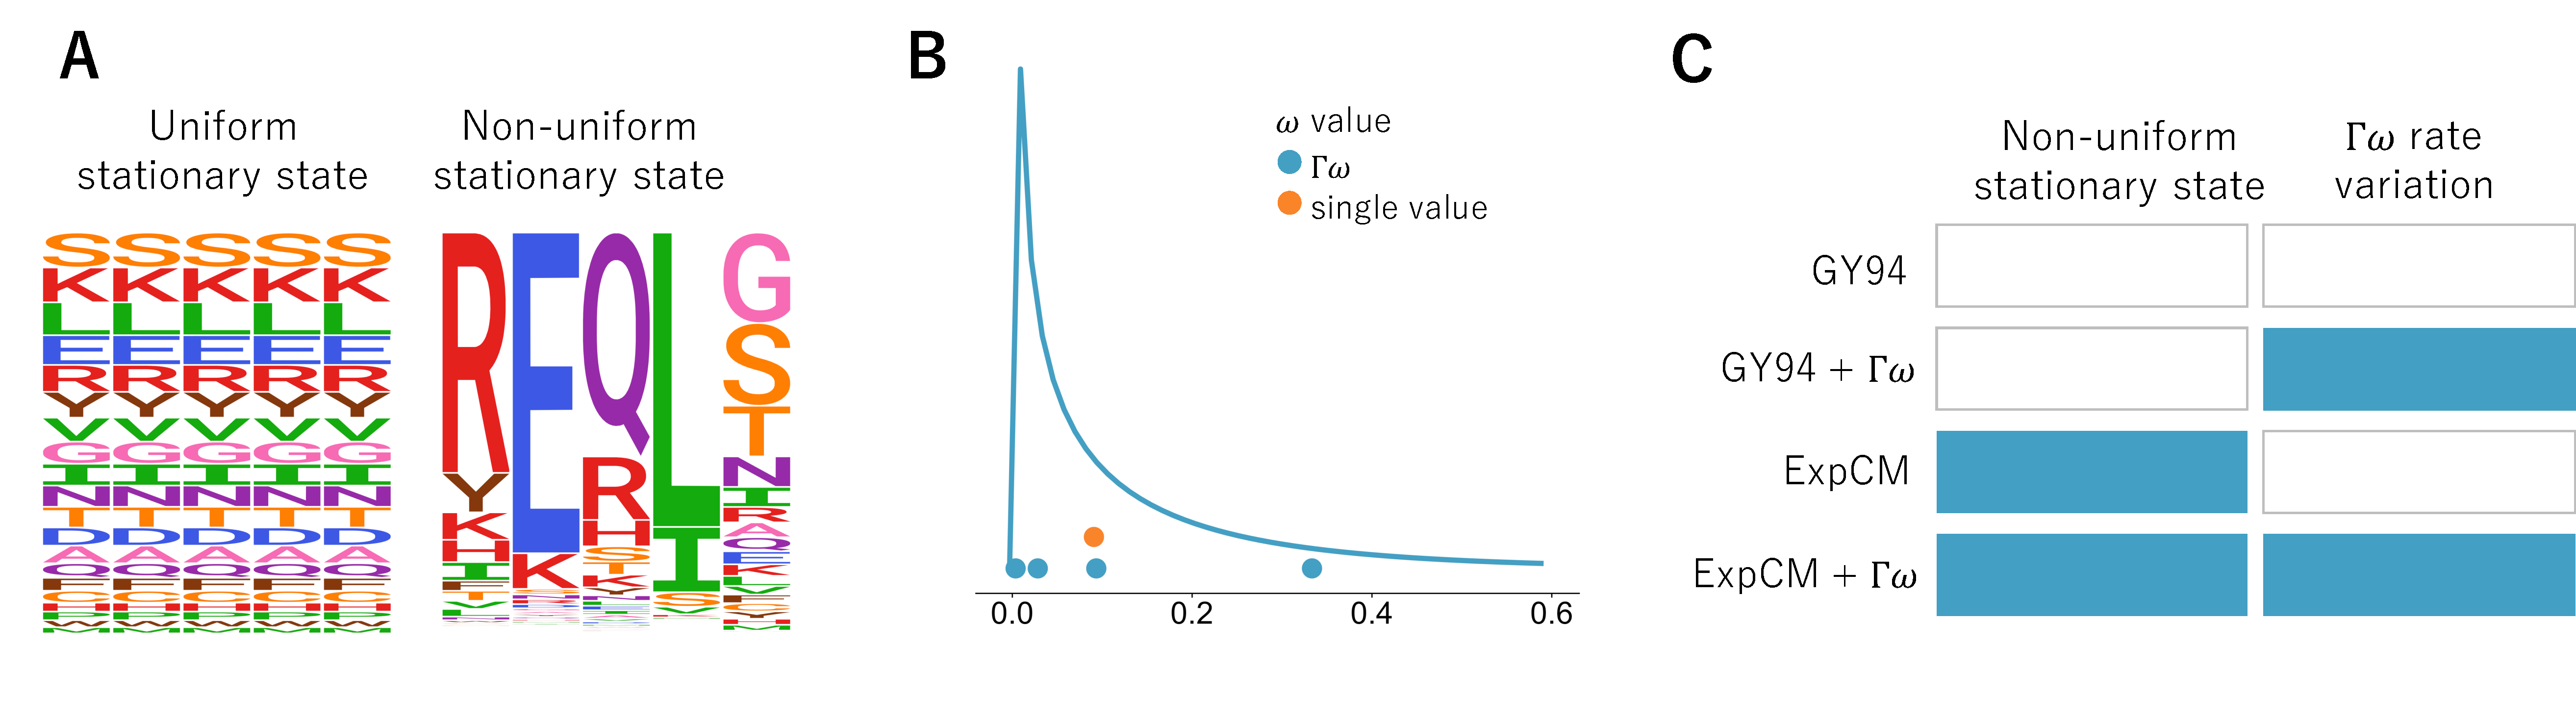
\includegraphics[width=0.90\textwidth]{figures/model_feature.pdf}}
\caption{\label{fig:model_feature}
\textbf{Comparison of substitution model features.}
Site-specific amino-acid profiles and $\Gamma$-distributed rate variation are both substitution model features which have been shown or theorized to lengthen branches. 
The models YNGKP M0, YNGKP M5, ExpCM, and ExpCM+$\Gamma\omega$ represent all possible combinations of these two features. 
Blue indicates presence and white indicates absence of a feature. 
from \ref{tab:wsn_low_params}
}
\end{figure}

\skhcomment{Section Outline:}


\begin{itemize}
\item There are different strategies to account for purifying selection and site-to-site rate variation. 
\begin{itemize}
\item $\Gamma\omega$ rate variation 
\begin{itemize}
\item single parameter controlling relative rate of non-synonymous to synonymous substitutions can vary across sites following some statistical distribution (usually $\Gamma$)
\item very common 
\item practical implementation - discretized distribution with the mean of $K$ bins. 
\end{itemize}
\item stationary state
\begin{itemize}
\item Explicitly model each amino-acid frequency at each site in the protein 
\item a more mechanistic description, no arbitrary statistical distribution 
\item practical limitation - how do you estimate these parameters without overfitting the data? We use experimental measurements to define the parameters \textit{a priori}
\end{itemize}
\end{itemize}
\item We can compare the effect of a model feature ($\Gamma\omega$ rate variation or non-uniform stationary state) while controlling the presence/absence of the other feature using models from the ExpCM and GY94 families. 
\end{itemize}


\subsection*{Effect of stationary state and rate variation on branch length estimation}

\begin{figure}[H]
\centerline{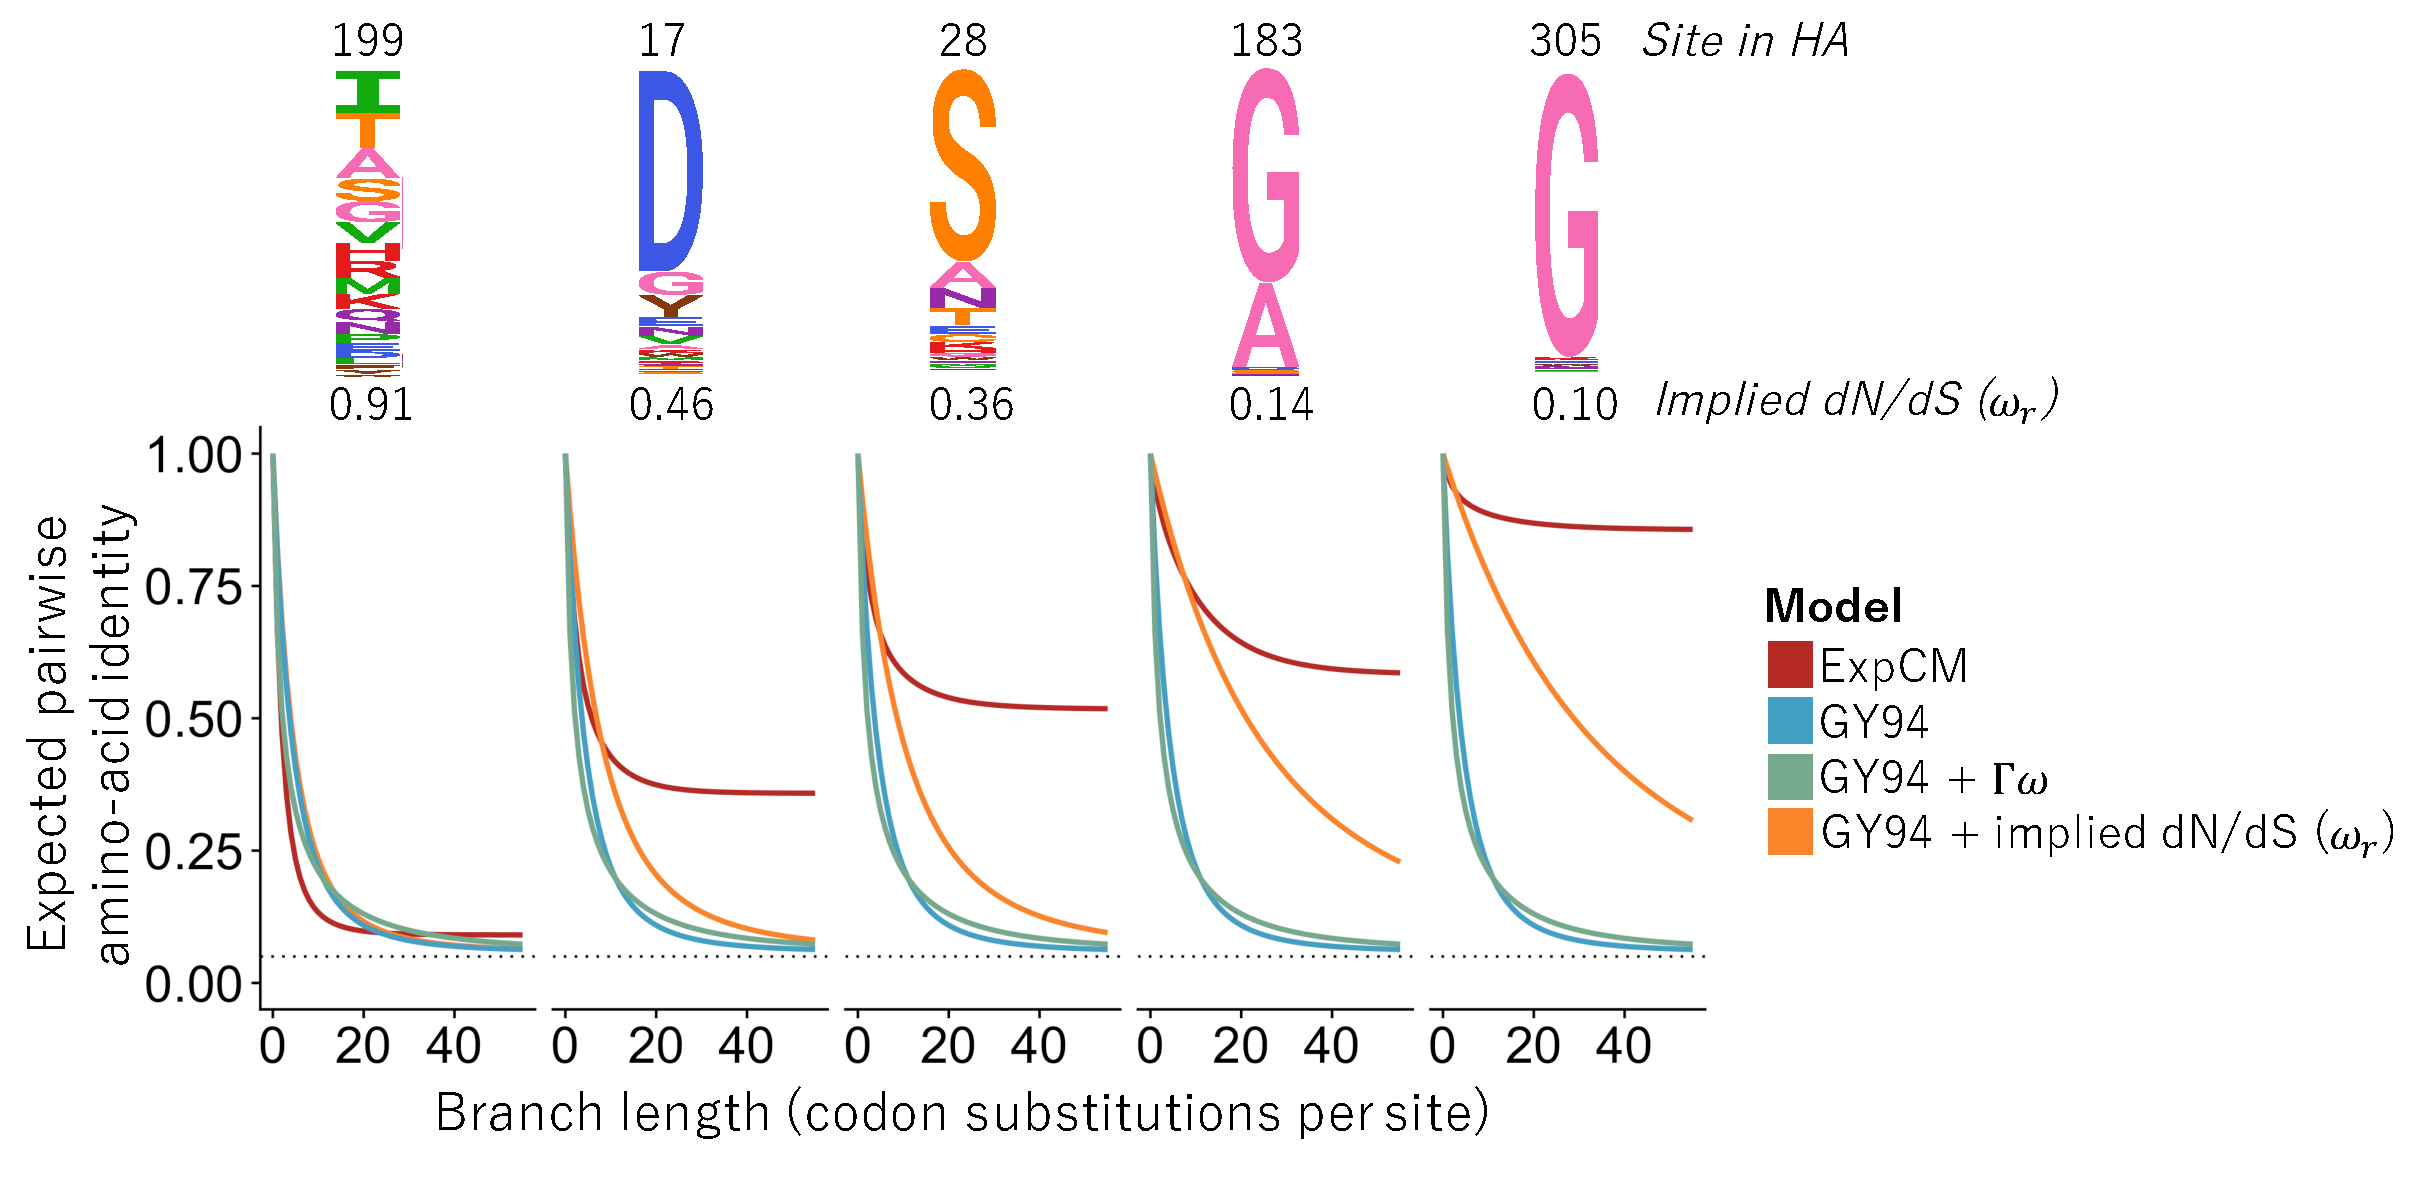
\includegraphics[width=0.90\textwidth]{figures/decay.pdf}}
\caption{\label{fig:decay}
\textbf{Effect of stationary state and rate variation on long branch estimation.}
The expected pairwise identity trajectories were calculated using \ref{eq:f} and models described in \ref{tab:wsn_low_params}.
The trajectories of the YNKGP M0 (blue) and YNGKP M5 (green) do not vary from panel to panel because neither model is site-specific. 
The deviation in trajectory of the ExpCM (red) from the YNGKP M0 (blue) increases from left to right as the mutational constraint of the amino-acid profile increases (logoplots, above). 
The deviation in trajectory of the YNGKP model with a site-specific $\omega$ value inferred from the ExpCM (yellow, \ref{eq:w_r}) is also positively correlated with the constraint of the site-specific amino-acid profiles but the effect size is smaller. 
}
\end{figure}

\skhcomment{Section Outline:}


\begin{itemize}
\item Substitution models are only useful for inferring branch lengths when they can accurately transform sequence divergence to time (branch length)
\item There is a saturation point in every substitution model where the temporal signal is lost (long tails in figure). 
\begin{itemize}
\item In the long tails the expected sequence divergence remains constant as time increases. 
\item The lost of temporal signal will affect long branches specifically.
\end{itemize}
\item Different model features (\ref{fig:model_feature}) can affect \textit{how long} it takes to reach the saturation point and the \textit{sequence divergence} at the saturation point 
\begin{itemize}
\item Adding $\Gamma\omega$ rate variation affects the ``path" to the saturation point but affects the sequence divergence at the saturation point minimally. Importantly, the saturation point is identically for every site in the protein. \skhcomment{These $\Gamma\omega$ parameters might not the best to show the effect of $\Gamma\omega$ on long branch estimation.} 
\item Adding a non-uniform stationary state creates a unique saturation point for each site in the protein. Sites which can tolerate many mutations have saturation points which are quite similar to the GY94 saturation point. However, constrained sites show a dramatic difference. 
\item This difference cannot be recapitulated by more complex modeling of the $\omega$ parameter. We can transform the GY94 model into a completely site-specific value by inferring a unique $\omega$ value from the ExpCM for each site in the protein. This model shows a substantial difference but does not recover the full effect of the ExpCM. 
\end{itemize}
\item No matter how ``well" you model site-to-site rate variation, you will underestimate \textit{very} long branches with a uniform stationary state. 
\end{itemize}

\subsection*{Failure to account for site-specificity leads to branch length underestimation.}

\begin{figure}[H]
\centerline{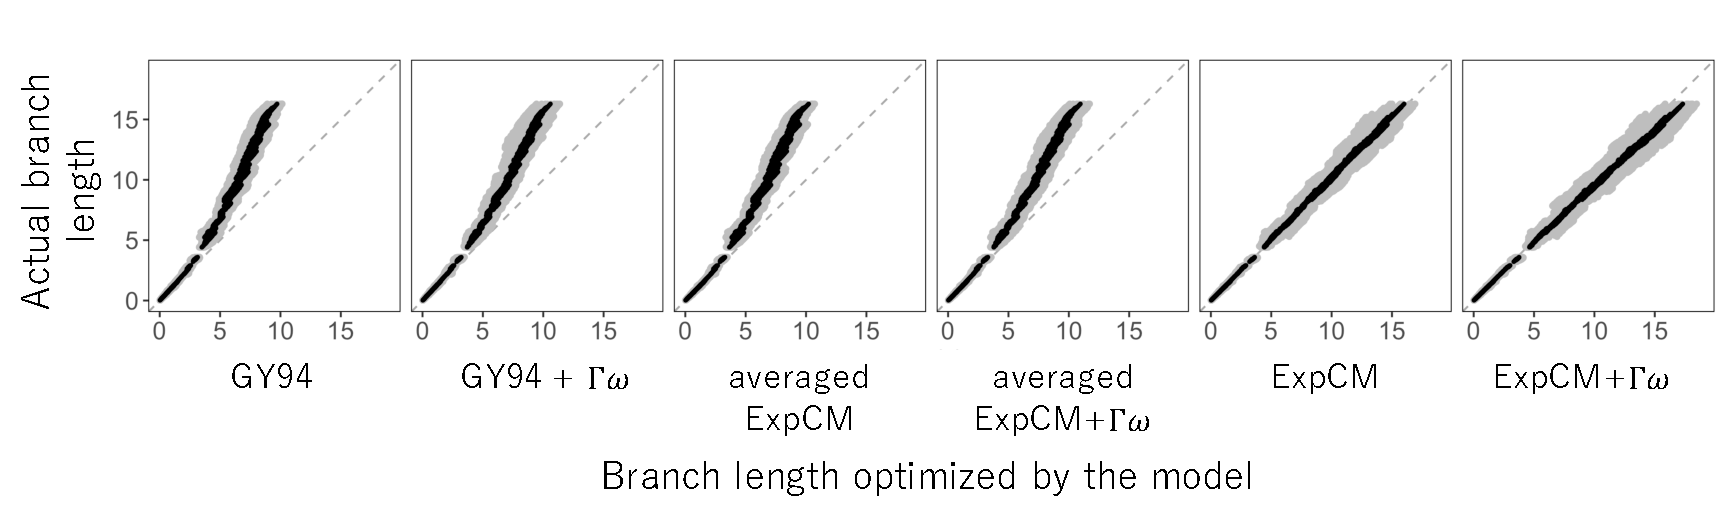
\includegraphics[width=0.85\textwidth]{figures/simulations}}
\caption{\label{simulations}
\textbf{Model performance under simulated, site-specific data.} 
\jdbcomment{Fonts are small, and tick labels definitely too small. I would show averaged.}
Alignments were simulated under an ExpCM (\ref{tab:sim_params}) along an HA tree and the branches were re-optimized by a model from the ExpCM or YNGKP family. 
The randomized ExpCMs have amino-acid profiles shuffled among the sites 
These randomized models are still site-specific but the relationship between the site and the experimental data is broken. 
Grey points represent the length of one branch and the black points are the mean branch lengths over eight simulations. 
The grey, dashed line is the reference line $y=x$, depicting the behavior of a model which is an unbiased estimator of the simulated branch length. 
}
\end{figure}

\skhcomment{Section Outline:}

\begin{itemize}
\item To test the effect of substitution model on data with site-specific amino acid frequencies, we simulated sequences under an ExpCM and re-inferred the branch lengths using different substitution models.
\item Uniform stationary state models underestimate long branches
\begin{itemize}
\item GY94 and GY94 + $\Gamma\omega$ both underestimate long branches 
\item The \textit{averaged} ExpCMs also underestimate long branches. These control models have uniform stationary states but still derive some information from the experiments. 
\item Non-uniform stationary state models accurately estimate long branches
\end{itemize}
\item If sequences have site-specific amino acid frequencies then non-uniform stationary state models, even with $\Gamma\omega$, will underestimate long branches.
\end{itemize}

\subsection*{empirical Data}

\begin{figure}[H]
\centerline{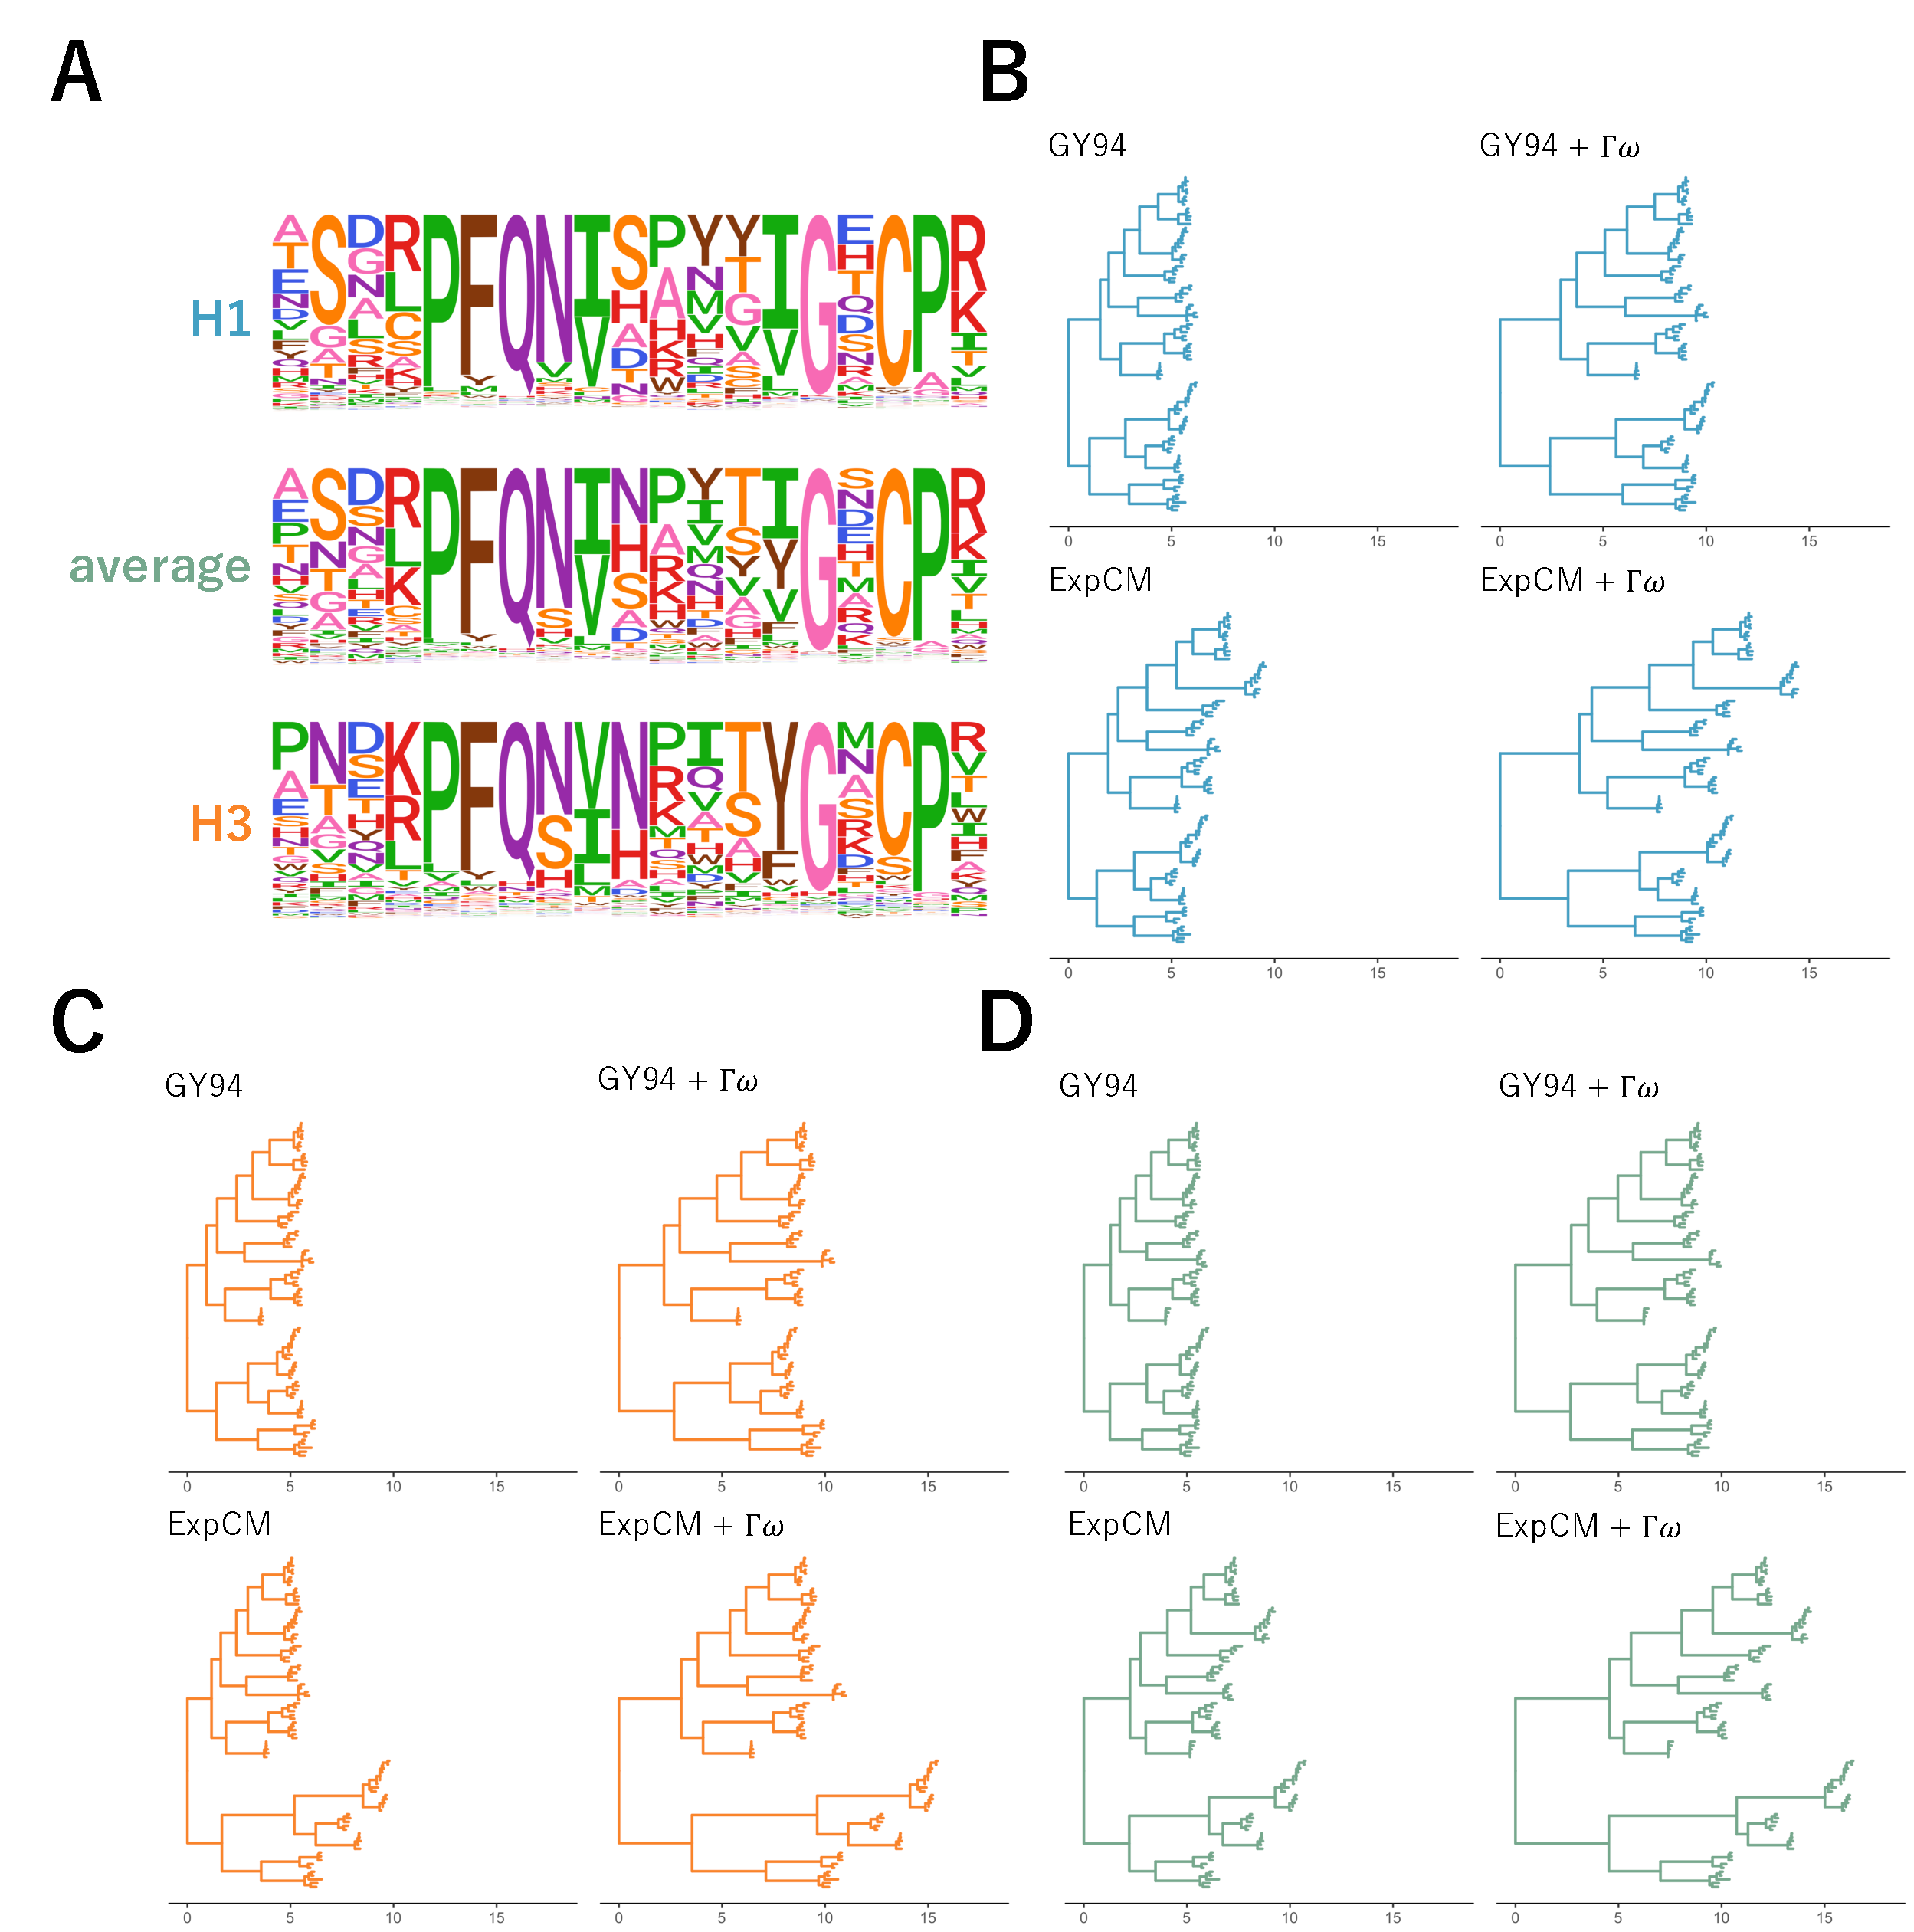
\includegraphics[width=0.9\textwidth]{figures/empirical_trees}}
\caption{\label{fig:empirical_trees}
\textbf{Trees optimized with an ExpCM defined by H1 preferences lengthen branches from the focal H1 sequence compared to YNGKP models.} 
\jdbcomment{Keep branch lengths in substitutions per site. Make a panel A show a prefs snippet, B H1 trees, C H3 trees, D H1+H3. Maybe increase very small font sizes a bit.}
The branch lengths of a base topology inferred using the GTR-CAT model were optimized by \textbf{(A)} an ExpCM defined by H1 preferences, \textbf{(B)} an ExpCM+$\Gamma\omega$ defined by H1 preferences, \textbf{(C)} YNKGP M0, and \textbf{(D)} YNGKP M5.
The branch lengths are normalized to the distance between A/South Carolina/1/1918 and A/Solomon Islands/3/2006 and colored to indicate the distance from the H1 focal sequence (black triangle).
}
\end{figure}


\skhcomment{Section Outline:}

\begin{itemize}
\item We tested the effect substitution model choice on branch length estimation using influenza HA sequences. 
\begin{itemize}
\item These sequences presumably evolve with site-specific frequencies but unlike the simulations we don't \textit{know} the model
\item These sequences are from fairly diverged proteins. Some sequences share only 40\% identity on the amino acid level 
\item HA has small, closely related subtypes with long branches between subtypes and groups. 
\end{itemize}
\item Both $\Gamma\omega$ and non-uniform stationary states result in an extension of branch lengths. 
\begin{itemize}
\item The addition of $\Gamma\omega$ extends branches independent of preferences. 
\item The addition of preferences extends branches \textit{from the focal sequence} independent of $\Gamma\omega$. 
\end{itemize}
\item The ExpCM does not have a uniform effect across the whole tree. 
\begin{itemize}
\item This is not too surprising. DMS makes accurate measurements in a given genetic background. 
\item You would expect epistatic effects over such a large divergence distance. ``Shifting preferences"
\end{itemize}
\end{itemize}

\subsection*{Competing effects of shifting preferences and long branches.}

\begin{figure}[H]
\centerline{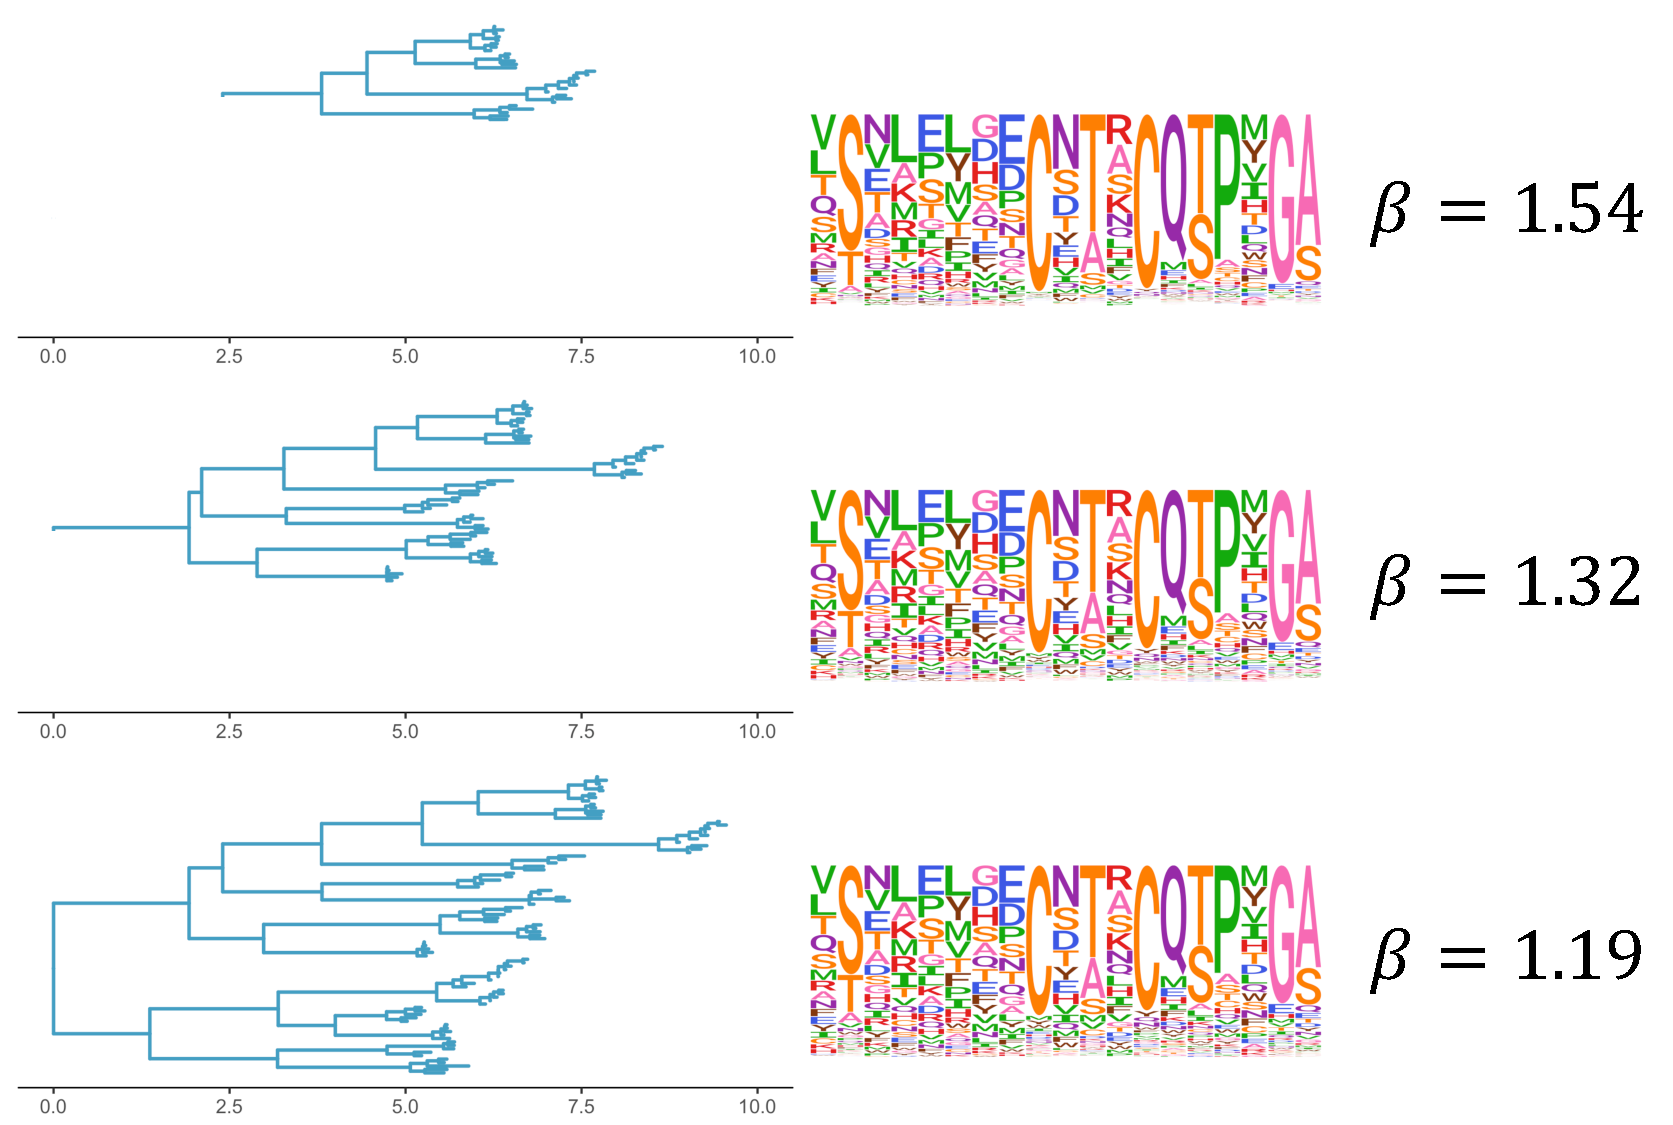
\includegraphics[width=0.85\textwidth]{figures/doud_compete_2}}
\caption{\label{fig:doud_compete}
\textbf{The ExpCM defined by H1 preferences lengthen longer branches on the HA tree.} 
\textbf{(A)} An HA alignment was subsampled to create three smaller alignments with varying degrees of divergence from the focal H3 sequence, referred to as "low", "intermediate", and "high". 
\textbf{(B)} The phylogenetic tree of the "high" alignment. 
The colors denote the alignment and the black circle denotes the focal H3 sequence. 
\textbf{(C)} The value of the ExpCM and ExpCM+$\Gamma\omega$ stringency parameter $\beta$ decreases as the divergence from the focal H3 sequence increases. 
\textbf{(D)} Comparisons of branch lengths optimized by the four substitution models for the varying degrees of divergence. 
Black points represent branches from the focal H3 sequence and grey points represent all other branches.  
The branch lengths are in average number of codon substitutions per site. 
}
\end{figure}


\begin{itemize}
\item We investigated the competing effects of shifting preferences and long branch estimation. That is, our preferences are most relevant to sequences they are close to but the effect of a non-uniform stationary is only observed on long branches. 
\begin{itemize}
\item We broke the large tree into small, sub trees with differing maximum divergence levels. 
\item We estimated the branch lengths using the same models we used for empirical data above. 
\end{itemize}
\item The ``relevance" of the preferences is inversely correlated with sequence divergence. 
\begin{itemize}
\item We used the ExpCM stringency parameter as the measure of preference ``relevance". The larger the $\beta$ value the more ``relevant" the preferences. 
\item As the maximum divergence of the tree increases the $\beta$ value decreases. 
\end{itemize}
\item All models estimate short branches relatively equally. 

\end{itemize}

\section*{Conclusion}

\begin{enumerate}
  \item We don't allow any of the models to vary by lineage. 
\end{enumerate}

\newpage
\section*{Materials and Methods}

\subsection*{Substitution models}
\subsubsection*{GY94 models}
\subsubsection*{ExpCMs}
We recap the \textbf{Exp}erimentally Informed \textbf{C}odon \textbf{M}odel (ExpCM) \citep{bloom2014experimentally,bloom2014informed,bloom2017identification,hilton2017phydms} to introduce nomenclature. 

In an ExpCM, rate of substitution $P_{r,xy}$ of site $r$ from codon $x$ to $y$ is written in mutation-selection form~\citep{halpern1998evolutionary,mccandlish2014modeling,spielman2015relationship} as
\begin{equation}
P_{r,xy} = Q_{xy} \times F_{r,xy}
\end{equation}
where $Q_{xy}$ is proportional to the rate of mutation from $x$ to $y$, and $F_{r,xy}$ is proportional to the probability that this mutation fixes.
The rate of mutation $Q_{xy}$ is assumed to be uniform across sites, and takes an HKY85-like~\citep{hasegawa1985dating} form:
\begin{equation}
Q_{xy} = 
\begin{cases}
\phi_w & \mbox{if $x$ and $y$ differ by a transversion to nucleotide $w$} \\
\kappa \phi_w & \mbox{if $x$ and $y$ differ by a transition to nucleotide $w$} \\
0 & \mbox{if $x$ and $y$ differ by $>1$ nucleotide.}
\end{cases}
\end{equation}
The $\kappa$ parameter represents the transition-transversion ratio, and the $\phi_w$ values give the expected frequency of nucleotide $w$ in the absence of selection on amino-acid substitutions, and are constrained by $1 = \sum_w \phi_w$.

The deep mutational scanning data are incorporated into the ExpCM via the $F_{r,xy}$ terms.
The experiments measure the preference $\pi_{r,a}$ of every site $r$ for every amino-acid $a$.
The $F_{r,xy}$ terms are defined in terms of these experimentally measured amino-acid preferences as
\begin{equation}
\label{eq:Frxy}
F_{r,xy} = 
\begin{cases}
   1 & \mbox{if $\mathcal{A}\left(x\right) = \mathcal{A}\left(y\right)$} \\
   \omega \times \frac{\ln\left[\left(\pi_{r,\mathcal{A}\left(y\right)} / \pi_{r,\mathcal{A}\left(x\right)}\right)^{\beta}\right]}{1 - \left(\pi_{r,\mathcal{A}\left(x\right)} / \pi_{r,\mathcal{A}\left(y\right)}\right)^{\beta}} & \mbox{if $\mathcal{A}\left(x\right) \ne \mathcal{A}\left(y\right)$}
   \end{cases}
\end{equation}
where $\mathcal{A}\left(x\right)$ is the amino-acid encoded by codon $x$, $\beta$ is the stringency parameter, and $\omega$ is the relative rate of nonsynonymous to synonymous substitutions after accounting for the amino-acid preferences.
The ExpCM has six free parameters (three $\phi_w$ values, $\kappa$, $\beta$, and $\omega$).
The preferences $\pi_{r,a}$ are \emph{not} free parameters since they are determined by an experiment independent of the sequence alignment being analyzed.

The ExpCM stationary state frequency $p_{r,x}$ of codon $x$ at site $r$ is~\citep{bloom2017identification} 
\begin{equation}
\label{eq:p_rx}
p_{r,x} = \frac{\left(\pi_{r,\mathcal{A}\left(x\right)}\right)^{\beta} \phi_{x_0} \phi_{x_1} \phi_{x_2}}{\sum_z \left(\pi_{r,\mathcal{A}\left(z\right)}\right)^{\beta} \phi_{z_0} \phi_{z_1} \phi_{z_2}},
\end{equation}
\subsection*{Theoretical effect of model choice on branch length}
\subsection*{Effect of model choice on natural sequences}

\subsubsection*{ExpCM + $\Gamma\omega$ and YNGKP M5}


\subsubsection*{Spielman $\omega_{r}$ values inferred from the ExpCM} 
We inferred the average nonsynonymous fixation rate from the ExpCM following~\citet{spielman2015relationship} as 
\begin{equation}
\label{eq:w_r}
\omega_{r} = \frac{\sum_{x} \sum_{y \in N_x} {p_{r,x} \times P_{r,xy}}}{\sum_{x} \sum_{y \in N_x} {p_{r,x} \times Q_{xy}}}
\end{equation}
where $p_{r,x}$ is the stationary state of the ExpCM at site $r$ and codon $x$, $P_{r,xy}$ is the substitution rate from codon $x$ to codon $y$ at site $r$, $Q_{xy}$ is the mutation rate from codon $x$ to codon $y$, and $N_x$ is the set of codons that are nonsynonymous to codon $x$ and differ from codon $x$ by only one nucleotide. 

\subsubsection*{Expected pairwise amino-acid identity}
\textit{Do I need to talk about the branchScale scaling I used?}
The expected pairwise amino-acid identity at a site $r$ over time $t$ for a given model is 
\begin{equation}
\label{eq:f}
\sum_a \sum_{x \in a} p_{r,x} \sum_{y \in a} [M_{r}\left(t\right)]_{xy}
\end{equation}
where $a$ is all amino acids, $p_{r,x}$ is the stationary state of the model at site $r$ and codon $x$, and $[M_{r}\left(t\right)]_{xy}$ is the transition rate from codon $x$ to codon $y$ at site $r$ given time $t$. 

\newpage
\section*{Supplemental Information}

\subsection*{Model Parameters for the simulations}

\begin{suppfig}[H]
\centerline{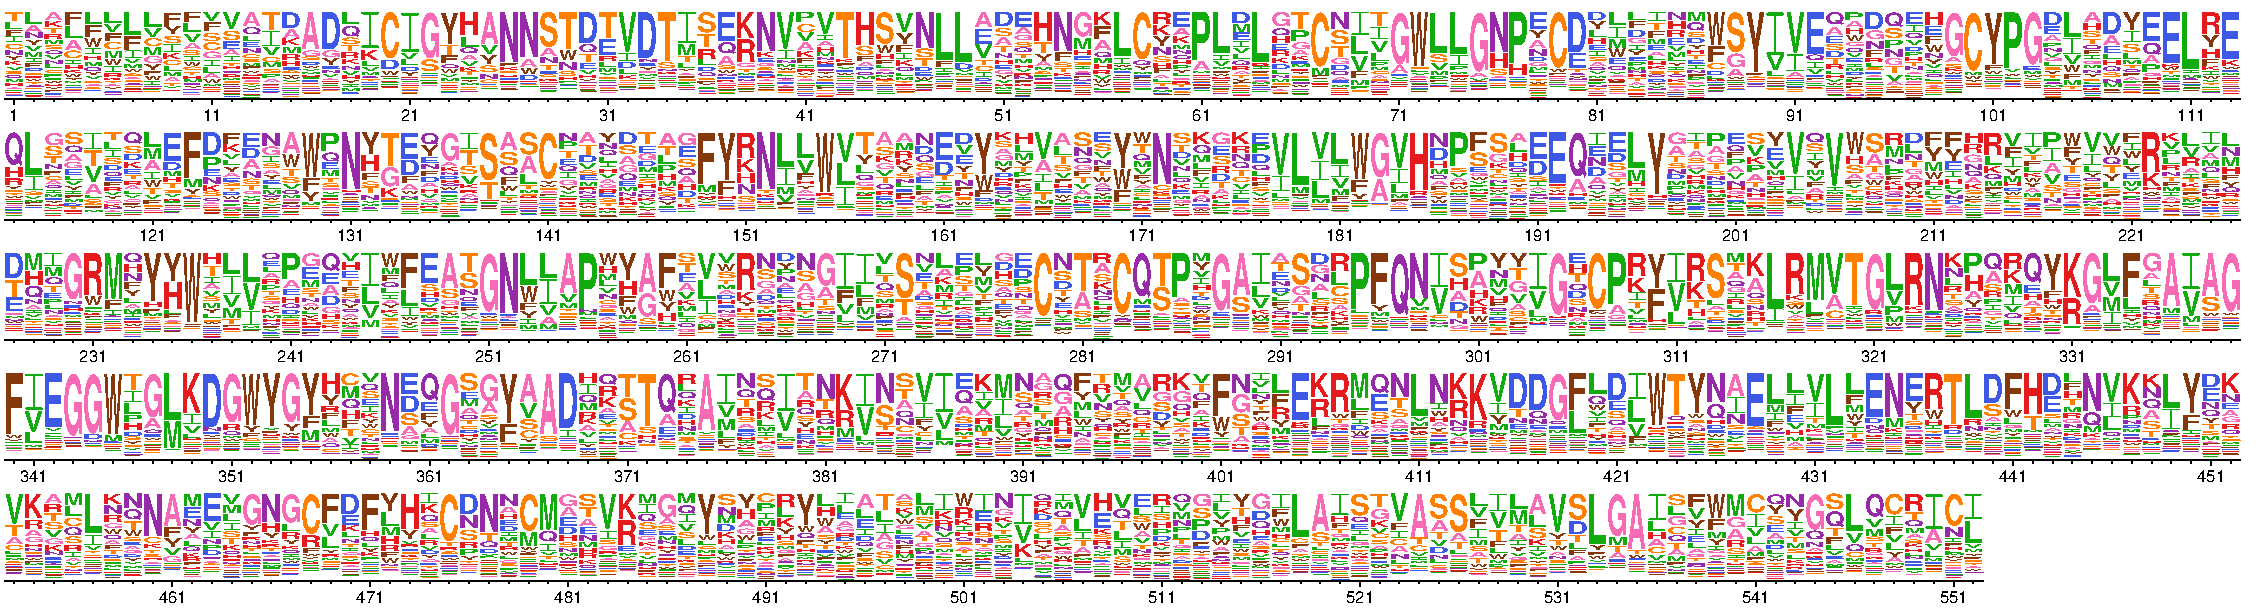
\includegraphics[width=\textwidth]{figures/prefs_doud}}
\caption{\label{suppfig:prefs_doud}
\textbf{H1 preferences measured by \cite{doud2016accurate} rescaled with the ExpCM stringency parameter optimized in \ref{fig:tree_doud}A  ($\beta = 1.19$)} 
\skhcomment{I need to change the $\beta$ value when the new \texttt{phydms} results finish running.}
}
\end{suppfig}

\begin{suppfig}[H]
\centerline{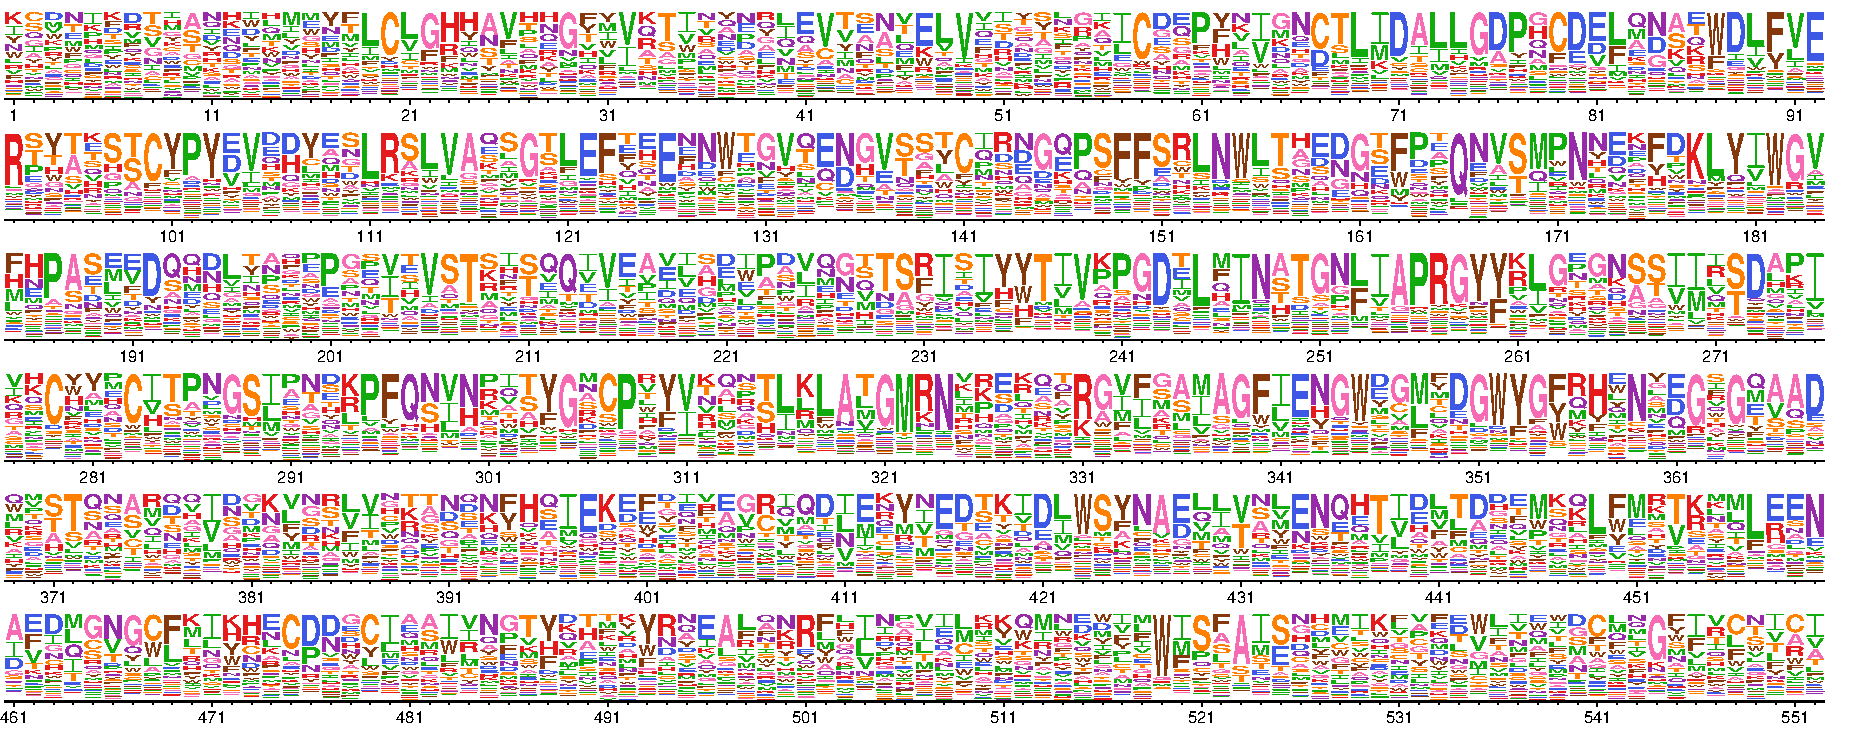
\includegraphics[width=\textwidth]{figures/prefs_lee}}
\caption{\label{suppfig:prefs_lee}
\textbf{H3 preferences measured by \textit{lee} rescaled with the ExpCM stringency parameter optimized in \ref{fig:tree_lee}A  ($\beta = 1.46$)}
\skhcomment{I need to change the $\beta$ value when the new \texttt{phydms} results finish running.} 
}
\end{suppfig}

\begin{figure}[H]
\centerline{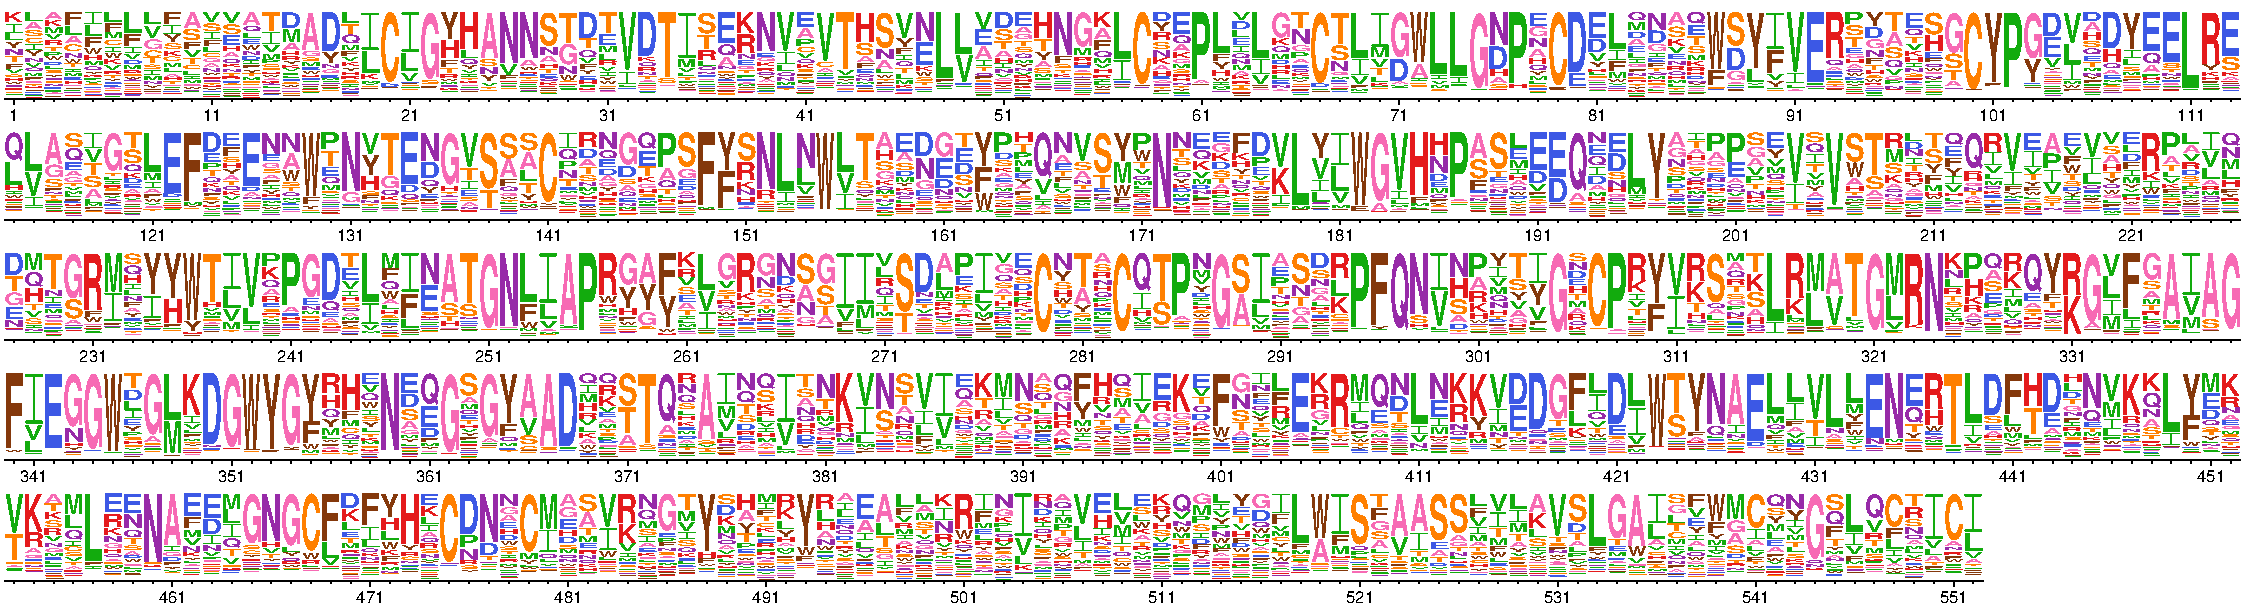
\includegraphics[width=\textwidth]{figures/prefs_average}}
\caption{\label{fig:prefs_average}
\textbf{The average of the H1 preferences measured by \cite{doud2016accurate} and the H3 preferences measured by \textit{Lee} rescaled with the ExpCM stringency parameter optimized in \ref{fig:tree_average}A  ($\beta = 1.77$)}}
\skhcomment{I need to change the $\beta$ value when the new \texttt{phydms} results finish running.}
\end{figure}



\begin{table}[t!]
\caption{\label{tab:simulation_params}
ExpCM parameters used to simulate sequences in Fig.~\ref{fig:simulation}.}
      \begin{tabular}{ccccc}
        \hline
          Parameter & Value\\ \hline
       	$\beta$ & $1.54$\\
	$\kappa$ & $3.60$\\
	$\omega$ & $0.20$\\
	$\phi_A$, $\phi_C$, $\phi_G$& $0.38$, $0.17$, $0.23$\\
      \end{tabular}
\end{table}

\begin{table}[t!]
\caption{\label{tab:wsn_low_params}
Model parameters used in  Fig.~\ref{fig:decay}.}
      \begin{tabular}{ccccc}
        \hline
          Model & Parameters\\ \hline
          ExpCM & $\beta=1.54196$\\
           & $\kappa=3.47184$\\
           & $\omega=0.219225$\\ 
          YNGKP M0 & $\kappa=2.9984$\\
          & $\omega=0.09076$\\
          YNGKP M5 & $\kappa=2.9984$\\
          & $\omega=0.09076$\\
      \end{tabular}
\end{table}

\begin{suppfig}[H]
\centerline{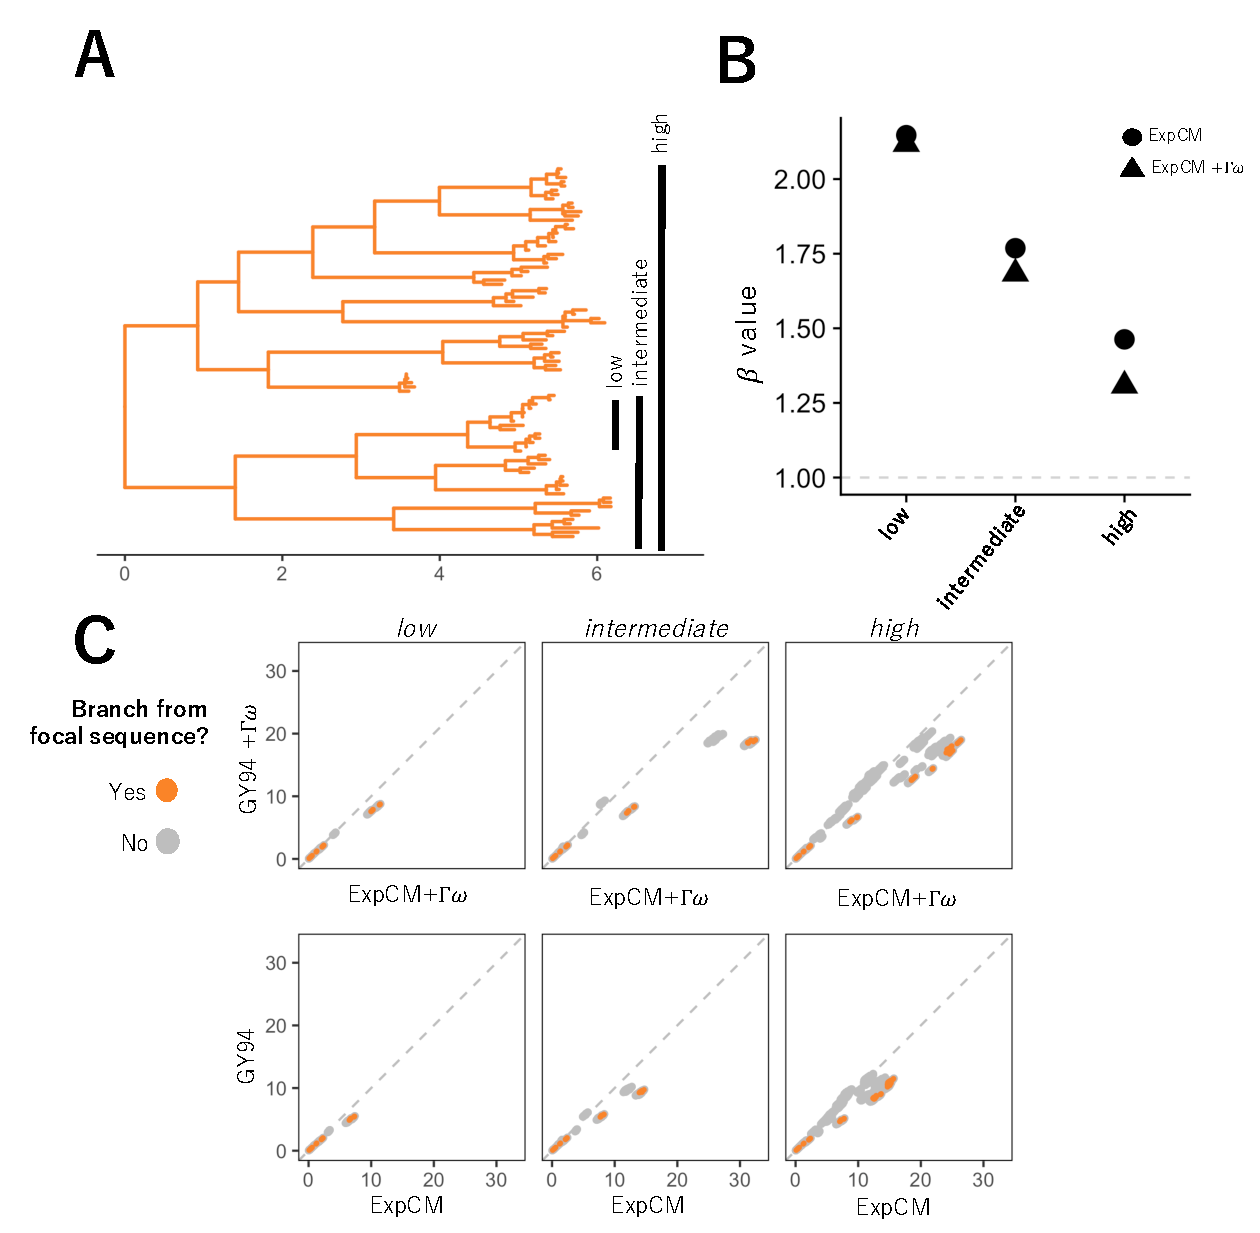
\includegraphics[width=0.85\textwidth]{figures/lee_compete}}
\caption{\label{fig:lee_compete}
\textbf{The ExpCM defined by H1 preferences lengthen longer branches on the HA tree.} 
\textbf{(A)} An HA alignment was subsampled to create three smaller alignments with varying degrees of divergence from the focal H3 sequence, referred to as "low", "intermediate", and "high". 
\textbf{(B)} The phylogenetic tree of the "high" alignment. 
The colors denote the alignment and the black circle denotes the focal H3 sequence. 
\textbf{(C)} The value of the ExpCM and ExpCM+$\Gamma\omega$ stringency parameter $\beta$ decreases as the divergence from the focal H3 sequence increases. 
\textbf{(D)} Comparisons of branch lengths optimized by the four substitution models for the varying degrees of divergence. 
Black points represent branches from the focal H3 sequence and grey points represent all other branches.  
The branch lengths are in average number of codon substitutions per site. 
}
\end{suppfig}


\clearpage 
\bibliographystyle{mbe}
\bibliography{references.bib}



\end{document}